\section{La représentation de la vitesse}

\begin{questions}
	\question Trajectoire du ballon : 
	\begin{center}
		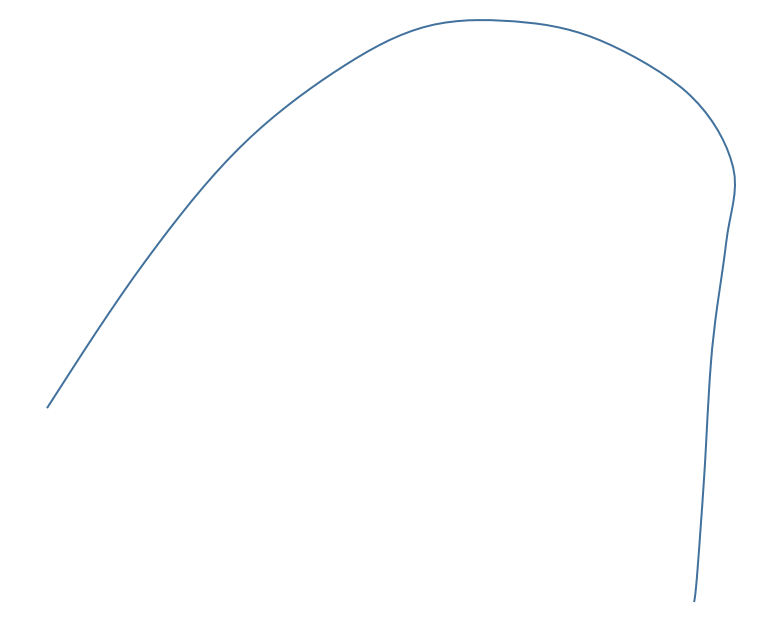
\includegraphics[scale=0.4]{traj1}
	\end{center}

	\question
	
		\begin{parts}
			\part La longueur des segments fléchés correspond à la valeur de la vitesse.
			
			\part La direction des segments fléchés est tangente à la trajectoire du ballon.
			
			\part Le sens du segment fléché indique le sens du trajet du ballon.
			
			\part \ \\
				\begin{center}
					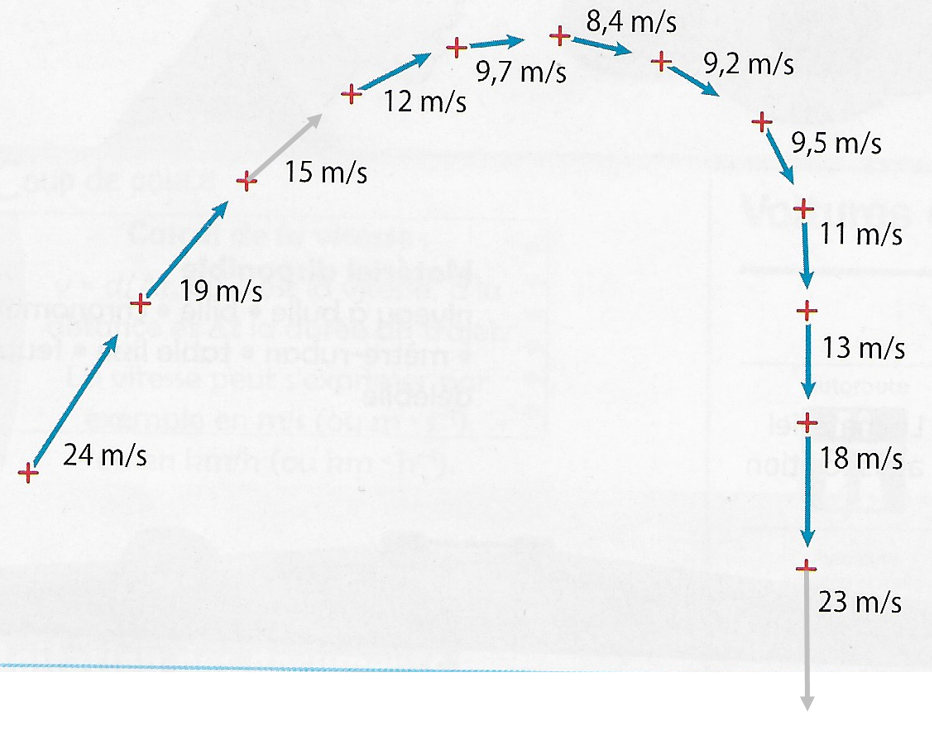
\includegraphics[scale=0.4]{traj2}
				\end{center}
		\end{parts}
\end{questions}